\newpage
\subsection{Reconstruction filters}
\label{sec:rfilters}
Image reconstruction filters are responsible for converting a series of radiance samples generated
jointly by the \emph{sampler} and \emph{integrator} into the final output image that will be written
to disk at the end of a rendering process.
This section gives a brief overview of the reconstruction filters that are available in Mitsuba.
There is no universally superior filter, and the final choice depends on a trade-off between
sharpness, ringing, and aliasing, and computational efficiency.

Desireable properties of a reconstruction filter are that it sharply captures all of the details that
are displayable at the requested image resolution, while avoiding aliasing and ringing. Aliasing is
the incorrect leakage of high-frequency into low-frequency detail, and ringing denotes oscillation artifacts
near discontinuities, such as a light-shadow transiton.

\begin{description}
\item[Box filter (\code{box}):]
the fastest, but also about the worst possible
reconstruction filter, since it is extremely prone to aliasing.
It is included mainly for completeness, though some rare situations
may warrant its use.
\item[Tent filter (\code{tent}):]
Simple tent, or triangle filter. This reconstruction filter never
suffers from ringing and usually causes less aliasing than a naive
box filter. When rendering scenes with sharp brightness discontinuities,
this may be useful; otherwise, negative-lobed filters will be preferable
(e.g. Mitchell-Netravali or Lanczos Sinc)

\item[Gaussian filter (\code{gaussian}):]
this is a windowed Gaussian filter with configurable standard deviation.
It produces pleasing results and never suffers from ringing, but may
occasionally introduce too much blurring.
When no reconstruction filter is explicitly requested, this is the default
choice in Mitsuba.
\item[Mitchell-Netravali filter (\code{mitchell}):]
Separable cubic spline reconstruction filter by Mitchell and Netravali
\cite{Mitchell:1988:Reconstruction}
This is often a good compromise between sharpness and ringing.

The plugin has two \code{float}-valued parameters named \texttt{B} and \texttt{C} that
correspond to the two parameters in the original research paper. By default, these
are set to the recommended value of $1/3$, but can be tweaked if desired.

\item[Catmull-Rom filter (\code{catmullrom}):]
This is a special version of the Mitchell-Netravali filter that has the
constants \texttt{B} and \texttt{C} adjusted to produce higher sharpness at the
cost of increased susceptibility to ringing.

\item[Lanczos Sinc filter (\code{lanczos}):]
This is a windowed version of the theoretically optimal low-pass filter.
It is generally one of the best available filters in terms of producing sharp
high-quality output. Its main disadvantage is that it produces strong ringing around
discontinuities, which can become a serious problem when rendering bright objects
with sharp edges (for instance, a directly visible light source will have black
fringing artifacts around it).
This is also the computationally slowest reconstruction filter.

This plugin has an \code{integer}-valued parameter named \code{lobes}, that
sets the desired number of filter side-lobes. The higher, the closer
the filter will approximate an optimal low-pass filter, but this also
increases the susceptibility to ringing. Values of 2 or 3 are common (3 is the default).
\end{description}
The next section contains a series of comparisons between reconstruction filters. In the first
case, a very high-resolution input image (corresponding to a hypothetical radiance field
incident at the camera) is reconstructed at low resolutions.

\newpage
\subsubsection{Reconstruction filter comparison 1: frequency attenuation and aliasing}
\vspace{-2mm}
Here, a high frequency function is reconstructed at low resolutions. A good filter
(e.g. Lanczos Sinc) will capture all oscillations that are representable at the desired
resolution and attenuate the remainder to a uniform gray. The filters are ordered by their
approximate level of success at this benchmark.
\renderings{
	\subfloat[A high resolution input image whose frequency decreases
	towards the borders. If you are looking at this on a computer, you may
	have to zoom in.]{\fbox{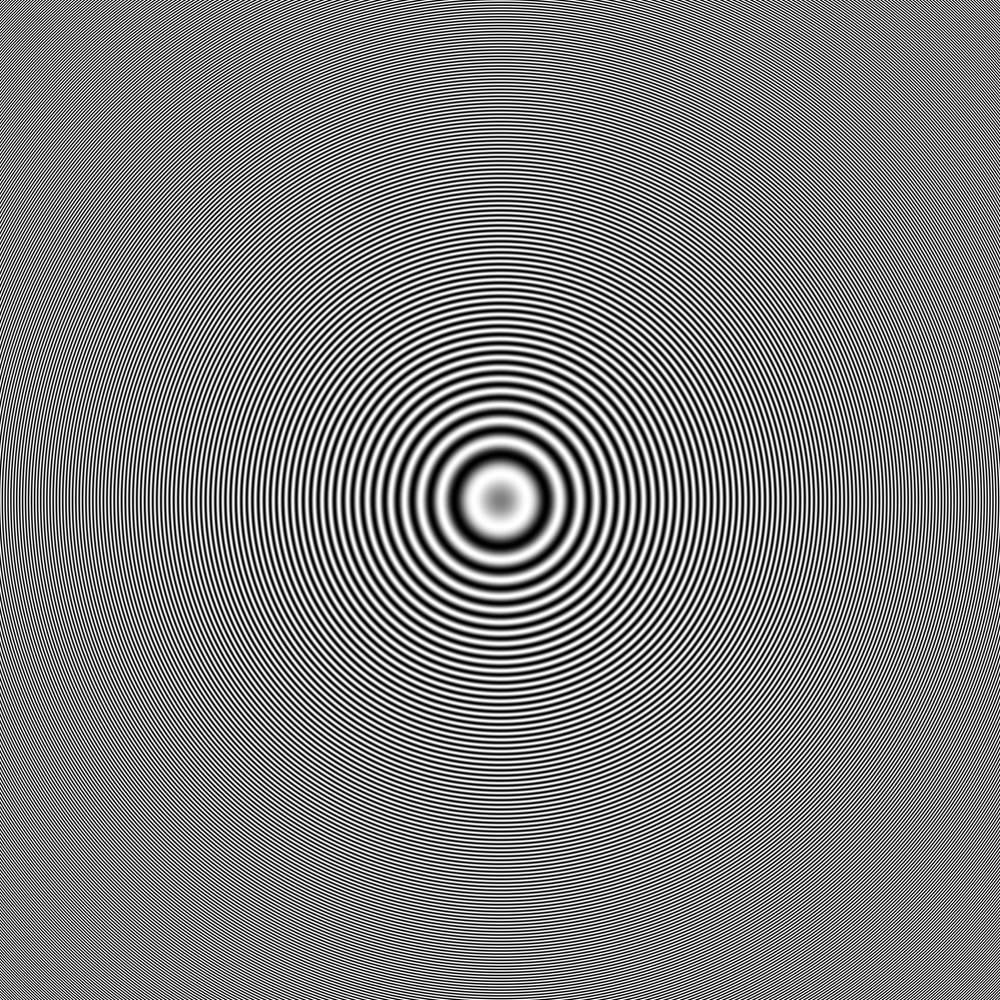
\includegraphics[width=0.43\textwidth]{images/rfilter_sines_input}}}
	\hfill
}
\vspace{-4mm}
\renderings{
	\medrendering{Box filter}{rfilter_sines_box}
	\medrendering{Tent filter}{rfilter_sines_tent}
	\medrendering{Gaussian filter}{rfilter_sines_gaussian}
}
\vspace{-4mm}
\renderings{
	\setcounter{subfigure}{3}
	\medrendering{Mitchell-Netravali filter}{rfilter_sines_mitchell}
	\medrendering{Catmull-Rom filter}{rfilter_sines_catmullrom}
	\medrendering{Lanczos Sinc filter}{rfilter_sines_lanczos}
}
\newpage
\subsubsection{Reconstruction filter comparison 2: ringing}
This comparison showcases the ringing artifacts that can occur when the rendered
image contains extreme and discontinuous brightness transitions. The
Mitchell-Netravali, Catmull-Rom, and Lanczos Sinc filters are affected by this problem.
Note the black fringing around the light source in the cropped Cornell box renderings below.
\renderings{
	\rendering{Box filter}{rfilter_cbox_box}
	\rendering{Tent filter}{rfilter_cbox_tent}
}
\vspace{-4mm}
\renderings{
	\setcounter{subfigure}{2}
	\rendering{Gaussian filter}{rfilter_cbox_gaussian}
	\rendering{Mitchell-Netravali filter}{rfilter_cbox_mitchell}
}
\vspace{-4mm}
\renderings{
	\setcounter{subfigure}{4}
	\rendering{Catmull-Rom filter}{rfilter_cbox_catmullrom}
	\rendering{Lanczos Sinc filter}{rfilter_cbox_lanczos}
}
\subsubsection{Specifying a reconstruction filter}
To specify a reconstruction filter, it must be instantiated inside
the sensor's film. Below is an example:
\begin{xml}
<scene version=$\MtsVer$>
	<!-- ... scene contents ... -->

	<sensor type="... sensor type ...">
		<!-- ... sensor parameters ... -->

		<film type="... film type ...">
			<!-- ... film parameters ... -->

			<!-- Instantiate a Lanczos Sinc filter with two lobes -->
			<rfilter type="lanczos">
				<integer name="lobes" value="2"/>
			</rfilter>
		</film>
	</sensor>
</scene>
\end{xml}
